\subsection{Interpolated Model}
The interpolated model methodology was developed using the "old" grid of phase diversity data. We have two sets of points: "on-grid" points that are spaced $\sim$every 100 pixels in x and y, and "off-grid" points that comprise the rest of the data. These two sets of data are depicted below. The "on-grid" points were used to develop the interpolated model in Zernike space, and the "off-grid" points were modeled and compared to the extracted Zernike coefficients.

\begin{figure}[h!]
\begin{center}
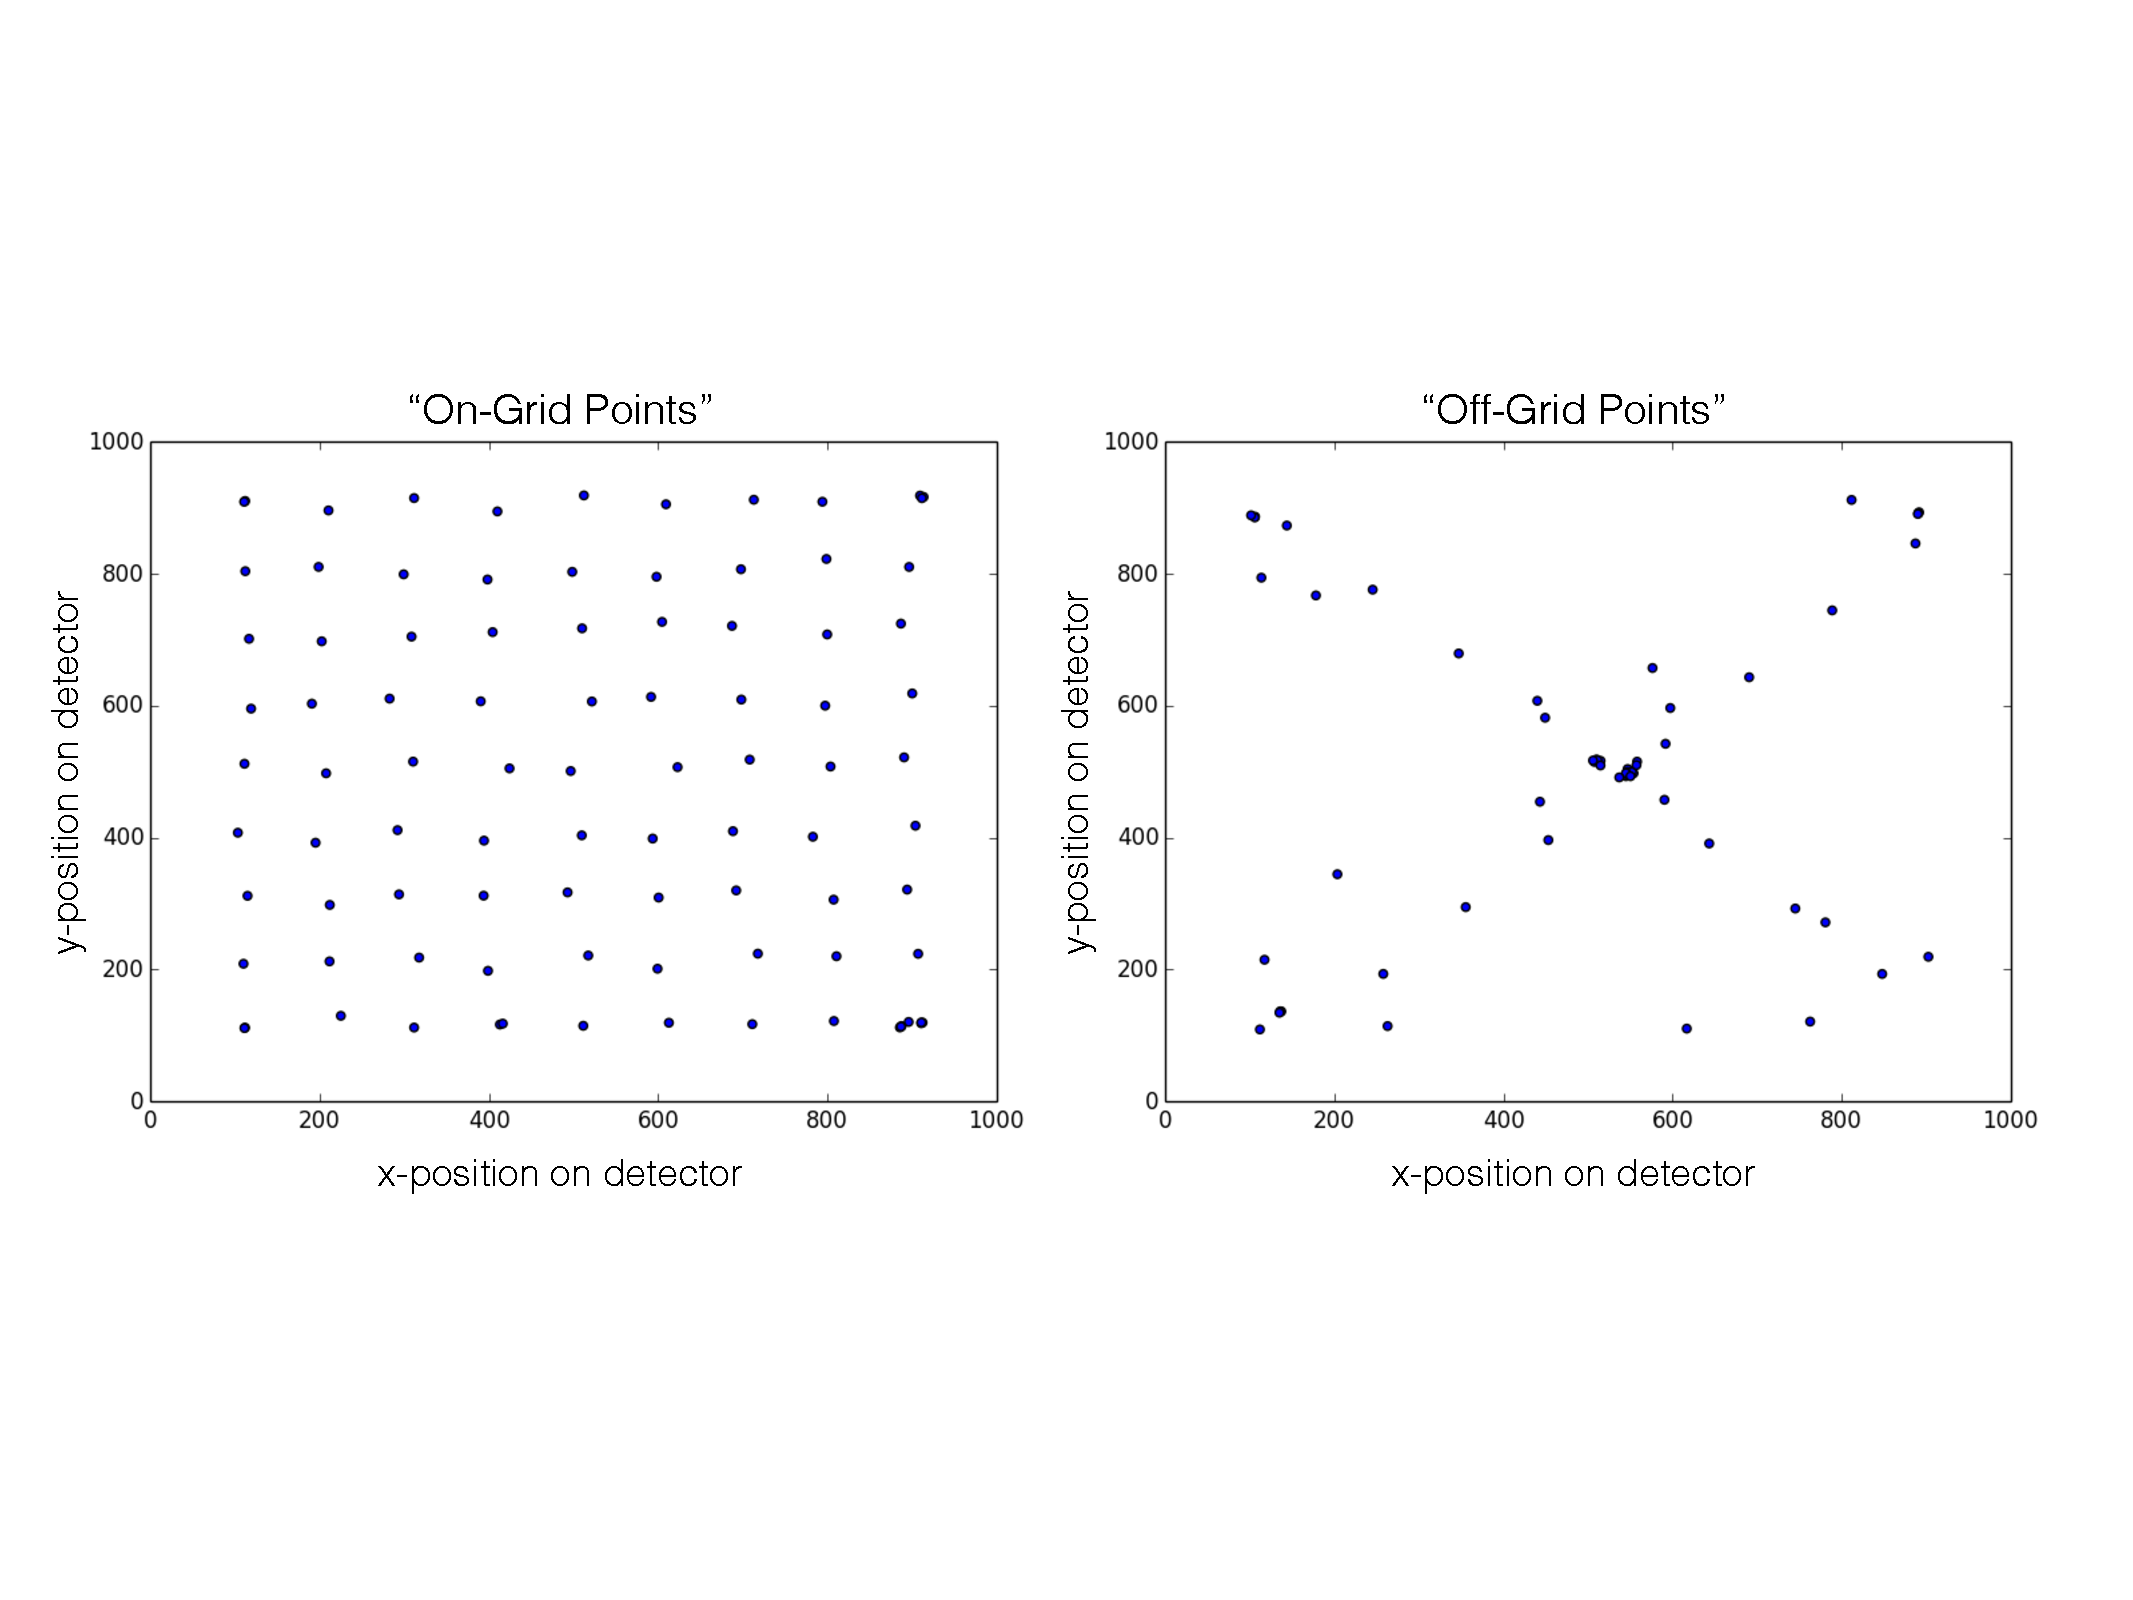
\includegraphics[width=0.7\columnwidth]{figures/on_off_grid_fig.pdf}
\caption{\textit{Left}: "On-grid" points utilized to generate the third-order spline interpolated model. \textit{Right}: "Off-grid" points used to test the fidelity of the model.}
\end{center}
\end{figure}

A third-order spline in $x$ and $y$ were used in create the model out to 200 Zernike terms. The third-order spline was chosen after modeling with a linear spline and the nearest neighbor; the third-order spline produced results that were more consistent with the extracted Zernike coefficients. 

As shown in the figure below, the off-grid Zernikes were well-modeled with the third-order spline interpolated model, with the exception of some defocus points at some of the positions and some astigmatism. However, overall, the recovery of the Zernike terms by this model is quite good with only about two-thirds of the data. 

A phase-map grid was delivered to the team using the third-order spline interpolated model with all of the old grid data ($\sim$ 150 data points) that is composed of 200 Zernike terms, which is more then sufficient to model a given phasemap based on the power spectrum. This will be used in \textit{StarFinder} 2.0.
  
  
  